%%%%%%%%%%%%%%%%%%%%%%%%%%%%%%%%%%%%%%%%%%%%%%%%%%%%%%%%%%%%%%%%%%%%%%%%%%%

\documentclass{standalone}

\usepackage{amsmath}
\usepackage{mathptmx}
\usepackage{pgfplots}
\usetikzlibrary{external}
\tikzexternalize{fantastic-tv-regression}
\pgfplotsset{compat=1.16}

%% IEEE uses Times Roman font, so we'll default to Times.
%% These three commands make up the entire times.sty package.
\renewcommand{\rmdefault}{ptm}
\renewcommand{\ttdefault}{pcr}
\normalfont\selectfont

\begin{document}

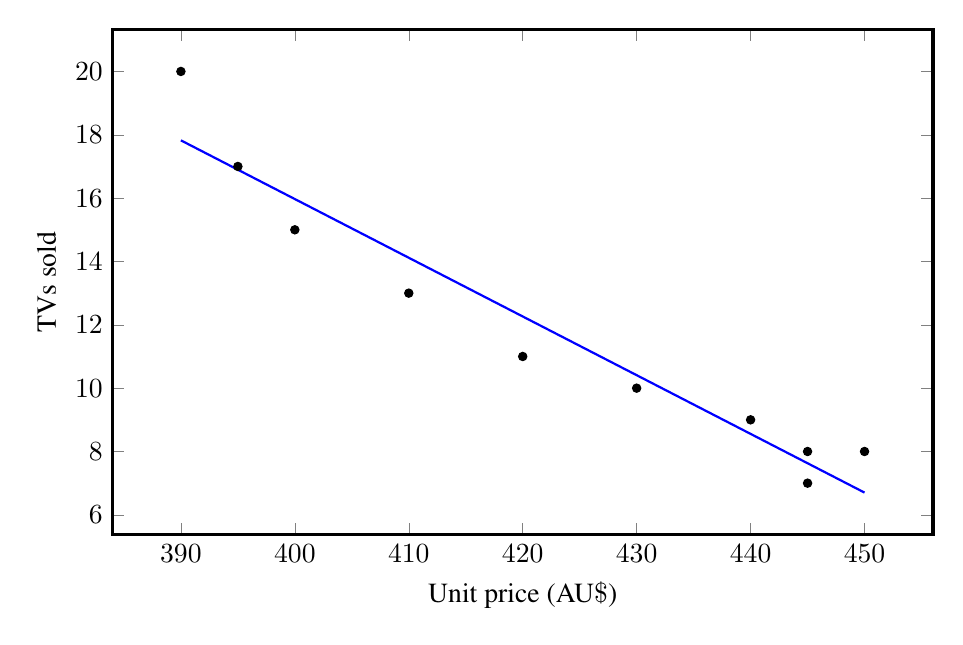
\begin{tikzpicture}
\tikzset{%%
  every mark/.append style={scale=1.0},%%
  scale=1.0%%
}
\pgfplotsset{%%
  every axis/.append style={font=\normalsize}%%
}
%%
\begin{axis}[%%
  axis line style=very thick,%%
  dotStyle/.style={only marks,mark size=1.5,black,mark color=black,mark=*},%%
  enlargelimits=true,%%
  height=8cm,%%
  plotStyle/.style={%%
    domain=390:450,%%
    mark=none,%%
    smooth,%%
    thick%%
  },%%
  width=12cm,%%
  %% x-axis
  xlabel={\normalsize Unit price~(AU$\$$)},%%
  xtick={%%
    390,400,410,420,430,440,450%%
  },%%
  xticklabels={%%
    $390$,$400$,$410$,$420$,$430$,$440$,$450$%%
  },%%
  %% y-axis
  ylabel={\normalsize TVs sold}%%
]
%%
%%
\addplot+ [plotStyle]
{-0.185366*x + 90.117073};
%%
\addplot[dotStyle] coordinates {
  (400,15)
  (445,8)
  (440,9)
  (410,13)
  (420,11)
  (430,10)
  (450,8)
  (445,7)
  (390,20)
  (395,17)
};
\end{axis}
\end{tikzpicture}

\end{document}
